\documentclass[tikz,border=0pt]{standalone}%
\usepackage{tikz-cd}
%\usepackage{silence}
\usetikzlibrary{arrows}
%\ErrorsOff*

\begin{document}
        %---------------------------------------------------------------
        %% Heaviside
        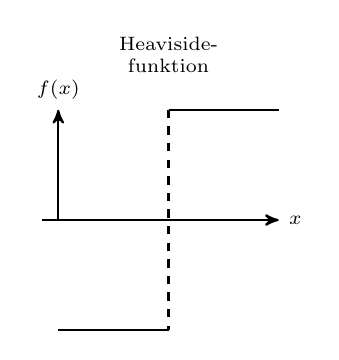
\begin{tikzpicture}[scale=.7,font=\scriptsize,thick,>=stealth']
            \coordinate (O) at (0,0);
            % horizontal axis
            \draw[->] (-0.3,0) -- (4,0) coordinate[label = {right:$x$}] (xmax);
            % vertical axis
            \draw[->] (0,0) -- (0,2) coordinate[label = {above:$f(x)$}] (ymax);
  
            \node[align=center] at (2,3) {Heaviside-\\funktion};
  
            \draw (2,2) -- (4,2);
            \draw (2,-2) -- (0,-2);
            \draw[dashed] (2,2) -- (2,-2);
        \end{tikzpicture}
        %---------------------------------------------------------------
        %% lineare Schwellwertfunktion
        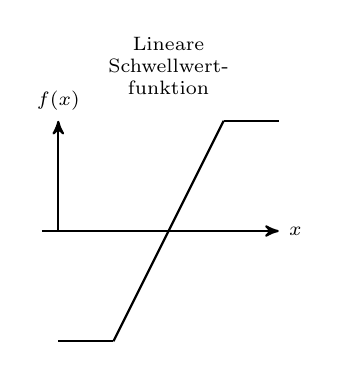
\begin{tikzpicture}[scale=.7,font=\scriptsize,thick,>=stealth']
            \coordinate (O) at (0,0);
            % horizontal axis
            \draw[->] (-0.3,0) -- (4,0) coordinate[label = {right:$x$}] (xmax);
            % vertical axis
            \draw[->] (0,0) -- (0,2) coordinate[label = {above:$f(x)$}] (ymax);
  
            \node[align=center] at (2,3) {Lineare\\Schwellwert-\\funktion};
  
            \draw (3,2) -- (4,2);
            \draw (1,-2) -- (0,-2);
            \draw (1,-2) -- (3,2);
        \end{tikzpicture}
        %---------------------------------------------------------------
        %% Fermifunktion
        \begin{tikzpicture}[scale=.7,font=\scriptsize,thick,>=stealth']
            \draw[white] (1,-2) -- (3,2);
            
            \draw[scale=.5,domain=-4:4,smooth,variable=\x,lightgray]      plot ({\x+4},{4*(1/(exp(-\x/.2)+1))});
            \draw[scale=.5,domain=-4:4,smooth,variable=\x,lightgray]      plot ({\x+4},{4*(1/(exp(-\x/.5)+1))});
            \draw[scale=.5,domain=-4:4,smooth,variable=\x,black]          plot ({\x+4},{4*(1/(exp(-\x/.8)+1))});
            % horizontal axis
            \draw[->] (-0.3,0) -- (4,0) coordinate[label = {right:$x$}] (xmax);
            % vertical axis
            \draw[->] (0,0) -- (0,2) coordinate[label = {above:$f(x)$}] (ymax);
            \node[align=center] at (2,3) {Logistische\\Funktion};
        \end{tikzpicture}
        %---------------------------------------------------------------
        %% Tangens Hyperbolicus
        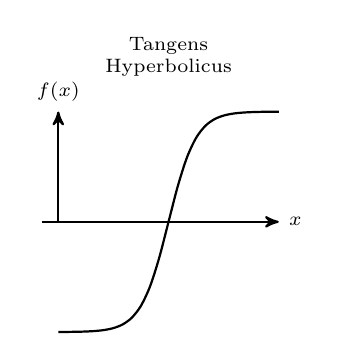
\begin{tikzpicture}[scale=.7,font=\scriptsize,thick,>=stealth']
            \coordinate (O) at (0,0);
            % horizontal axis
            \draw[->] (-0.3,0) -- (4,0) coordinate[label = {right:$x$}] (xmax);
            % vertical axis
            \draw[->] (0,0) -- (0,2) coordinate[label = {above:$f(x)$}] (ymax);
            \node[align=center] at (2,3) {Tangens\\Hyperbolicus};
            \draw[scale=0.5,domain=-4:4,smooth,variable=\x,black] plot ({\x+4},{4*tanh(\x)});
        \end{tikzpicture}
\end{document}